\documentclass[12pt]{article}
\usepackage{amsmath}
\usepackage{physics}
\usepackage{graphicx}

\author{Patryk Kozlowski}
\title{Homework 1}
\date{\today}
\begin{document}
\maketitle
\section{Problem 1}
Ashcroft and Mermin, Chapter 2, Problem 1
\subsection{Part a}
What is the relation between $n$ and $k_F$ in two dimensions?
\subsubsection{Solution}
By definition, the number of particles is an integral over the density of states that are singly occupied, i.e., up to the Fermi wave vector. In two dimensions, the density of states is given by
\begin{equation}
    N = \int_{0}^{k_F} \frac{d^2k}{(2\pi)^2}
\end{equation}
Expanding in polar coordinates, we have
\begin{equation}
    N = \int_{0}^{k_F} \int_{0}^{2\pi } \frac{d\theta}{(2\pi)^2} k \, dk = \frac{1}{2\pi}\int_{0}^{k_F} k \, dk = \frac{k_F^2}{4\pi}
\end{equation}
The particle density is defined as the number of particles per unit area. Since we have a unit area, then
\begin{equation}
    n = \frac{N}{A} = \frac{k_F^2}{4\pi}
\end{equation}
\subsection{Part b}
What is the relation between $k_F$ and $r_s$ in two dimensions?
\subsubsection{Solution}
The Wigner-Seitz radius is defined as the area per particle in real space. So in two dimensions, this is simply the area of a circle with radius $r_s$: $A = \pi r_s^2$. The particle density is defined as the number of particles per unit area. Since we have defined the area above, we can write
\begin{equation}
    n = \frac{N}{A} = \frac{N}{\pi r_s^2}  
\end{equation}
But then we also found that the particle density can be expressed in terms of the Fermi wave vector, so we have a relationship between the Wigner-Seitz radius and the Fermi wave vector
\begin{equation}
    n = \frac{k_F^2}{4\pi} = \frac{N}{\pi r_s^2} \implies k_F = \frac{2\sqrt{N}}{r_s}
\end{equation}
\subsection{Part c}
Prove that in two dimensions the free electron density of levels \( g(E) \) is a constant independent of \( \epsilon \) for \( \epsilon > 0 \), and 0 for \( \epsilon < 0 \). What is the constant?
\subsubsection{Solution}
A free electron only has the energy contribution from its kinetic part
\begin{equation}
    \epsilon = \frac{\hbar^2 k^2}{2m} \implies k = \sqrt{\frac{2m\epsilon}{\hbar^2}}
\end{equation}
Now the number of single particle states up to this momentum \( k \) is given as before
\begin{equation}
    N(k) = \int_{0}^{k} \frac{d^2k}{(2\pi)^2} = \frac{1}{(2\pi)^2} \int_{0}^{k} d^2k = \frac{k^2}{4\pi}
\end{equation}
The density of levels is defined by the derivative of the number with respect to the momentum, but we eventually want this in terms of the energy so we perform another derivative
\begin{equation}
    g(\epsilon) = \dv{N}{k} \dv{k}{\epsilon}
\end{equation}
First we evaluate the first derivative
\begin{equation}
    \dv{N}{k} = \frac{k}{2\pi}
\end{equation}
Then we find the derivative of the momentum with respect to the energy
\begin{equation}
    \dv{k}{\epsilon} = \dv{\sqrt{\frac{2m\epsilon}{\hbar^2}}}{\epsilon} = \frac{\sqrt{2m}}{\hbar} \times \frac{1}{2\sqrt{\epsilon}} = \frac{1}{2k} \times \frac{2m}{\hbar^2}
\end{equation}
Putting it all together, we find
\begin{equation}
    g(\epsilon) = \frac{k}{2\pi} \times \frac{1}{2k} \times \frac{2m}{\hbar^2} = \frac{m}{2\pi \hbar^2}
\end{equation}
We know that a free electron cannot have a negative energy, so we get the distribution
\begin{equation}
    g(\epsilon) = \begin{cases}
        \frac{m}{2\pi \hbar^2} \& \epsilon > 0 \\
        0 \& \epsilon < 0
    \end{cases}
\end{equation}
\subsection{Part d}
Show that because \( g(\epsilon) \) is constant, every term in the Sommerfeld expansion for \( n \) vanishes except the \( T = 0 \) term. Deduce that \( \mu = \epsilon_F \) at any temperature.

\subsubsection{Solution}
We know that
\begin{equation}
    \begin{aligned}
\int_{-\infty}^{\infty} \& H(\varepsilon) f(\varepsilon) d \varepsilon \\
\& = \int_{-\infty}^\mu H(\varepsilon) d \varepsilon + \frac{\pi^2}{6}\left(k_B T\right)^2 H^{\prime}(\mu) + \frac{7 \pi^4}{360}\left(k_B T\right)^4 H^{\prime \prime \prime}(\mu) + O\left(\frac{k_B T}{\mu}\right)^6
\end{aligned}
\end{equation}
and the particle density is given as
\begin{equation}
    n = \int_{-\infty}^{\infty} d \varepsilon \, g(\varepsilon) f(\varepsilon)
\end{equation}
Considering the equivalence between \( g(\epsilon) \) and \( H(\epsilon) \), we know that every higher order term in the expansion depends on some sort of derivative of the density of states, and because it is a constant, we know these terms turn out to be 0. Then, by the definition of the Fermi energy as the limit at which the fermion occupation numbers go from 0 to 1, one can make the simplification
\begin{equation}
    \int_{-\infty}^{\infty} H(\varepsilon) f(\varepsilon) d \varepsilon = \int_{-\infty}^{\epsilon_F} H(\varepsilon) d \varepsilon
\end{equation}
so we see through this Sommerfeld expansion, that we must have
\begin{equation}
    \int_{-\infty}^{\epsilon_F} H(\varepsilon) d \varepsilon = \int_{-\infty}^{\mu } H(\varepsilon) d \varepsilon
\end{equation}
, which implies that \( \mu = \epsilon_F \) at any temperature.
\subsection{Part e}
(e) Deduce from (2.67) that when \( g(\varepsilon) \) is as in (c), then
\[
\mu + k_B T \ln \left(1 + e^{-\mu  / k_B T}\right) = \varepsilon_F
\]
\subsubsection{Solution}
We are starting with the definition of the particle density
\begin{equation}
    n = \int_{-\infty}^{\infty} d \varepsilon \, g(\varepsilon) f(\varepsilon)
\end{equation}
The piece of information from the previous part is that we can approximate the density of states as constant, so we have \( g(\varepsilon) = g_0 = \frac{m}{2\pi \hbar^2} \). We know the form of the Fermi function as \( f(\varepsilon) = \frac{1}{1 + e^{\frac{\varepsilon - \mu}{k_B T}}} \), and it is 0 for negative energy values and also 0 for values greater than the Fermi energy. So we can write the integral as
\begin{equation}
    n = \frac{m}{2\pi \hbar^2}\int_{0}^{\infty} d \varepsilon \, \frac{1}{1 + e^{\frac{\varepsilon - \mu}{k_B T}}}
\end{equation}
To perform the integral

\[
\int_0^\infty \frac{1}{1 + e^{(\varepsilon - \mu) / (k_B T)}} \, d\varepsilon
\]

we use the substitution \( u = \frac{\varepsilon - \mu}{k_B T} \), which gives \( \varepsilon = u \cdot k_B T + \mu \), and \( d\varepsilon = k_B T \, du \). The limits of integration change accordingly: when \( \varepsilon = 0 \), \( u = -\frac{\mu}{k_B T} \), and as \( \varepsilon \to \infty \), \( u \to \infty \).

Substituting into the original integral, we get

\[
\int_{-\mu/(k_B T)}^{\infty} \frac{k_B T}{1 + e^u} \, du
\]

Factoring out the constant \( k_B T \), this becomes

\[
k_B T \int_{-\mu/(k_B T)}^{\infty} \frac{1}{1 + e^u} \, du
\]

The integral \( \int \frac{1}{1 + e^u} \, du \) is a standard result and evaluates to \( \ln(1 + e^u) \). Applying the limits of integration, we have

\[
k_B T \left[ \ln(1 + e^u) \right]_{-\mu/(k_B T)}^{\infty}
\]

At the upper limit \( u \to \infty \), \( \ln(1 + e^u) \to u \). At the lower limit \( u = -\frac{\mu}{k_B T} \), we get \( \ln(1 + e^{-\mu/(k_B T)}) \). Thus, 
\begin{equation}
    n = \frac{m}{2\pi \hbar^2} k_B T \left( \frac{\varepsilon - \mu}{k_B T} - \ln(1 + e^{-\mu/(k_B T)}) \right)
\end{equation}
We know that the particle number divided by the density of states is defined as the Fermi energy, so we have
\begin{equation}
    \varepsilon_F = k_B T \left( \frac{\varepsilon - \mu}{k_B T} - \ln(1 + e^{-\mu/(k_B T)}) \right) \implies \frac{\varepsilon_F}{k_B T} = \frac{\varepsilon - \mu}{k_B T} - \ln(1 + e^{-\mu / k_B T})
\end{equation}
\subsection{Part f}
\subsubsection{Solution}
We can make an approximation for the natural logarithm as $\ln(1+e^{-\mu/k_BT}) \approx e^{-\mu/k_BT}$, which is valid for $\mu \gg k_BT$. This defines the correction.
The Sommerfeld expansion relies on being able to approximate the behavior of integrals near the Fermi energy by expanding functions like the density of states in a power series around \(\varepsilon_F\). In 3D, where the density of states varies smoothly with energy, this works well.

In 2D, where the density of states is constant, this smooth variation doesn't exist, and therefore the Sommerfeld expansion breaks down. The low-temperature corrections in 2D are non-analytic, meaning the temperature dependence cannot be expressed as a simple power series in \(T\), unlike in higher dimensions.
\section{Problem 4}
Ashcroft \& Mermin, Chapter 4, Problem 5
\subsection{Part a}
\begin{figure}[h]
    \centering
    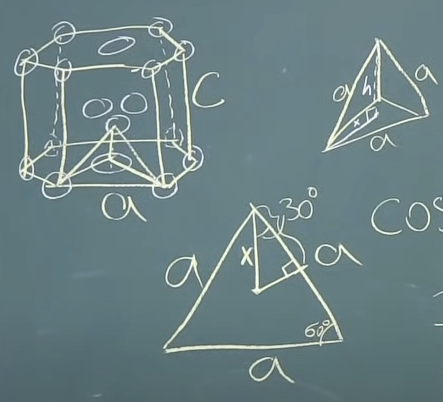
\includegraphics[width=0.5\textwidth]{hcp.png}
\end{figure}
As these diagrams show, using trigonometry we can get $\cos(30^\circ) = \frac{a}{2x}$, so $x = \frac{a}{\sqrt{3}}$. Since we know that the relation must hold with $h=\frac{c}{2}$:
\begin{equation}
    h^2+x^2 = a^2 \implies \left(\frac{c}{2}\right)^2 + \left(\frac{a}{\sqrt{3}}\right)^2 = a^2 \implies \frac{c^2}{4} + \frac{a^2}{3} = a^2 \implies \frac{c^2}{4} = \frac{2a^2}{3} \implies \left(\frac{c}{a}\right)^2 = \frac{8}{3} 
\end{equation}
And then we get the ideal ratio of $c/a = \sqrt{\frac{8}{3}} \approx 1.63$.
\subsection{Part b}
Let's start with the simple task of figuring out the density in the body-centered cubic arrangement. We know that the volume is given by $a^3$, where $a$ is the lattice constant, which in the cubic phase is 4.23 angstroms, suggesting that the volume of the unit cell is $4.23^3 = 76.2$ cubic angstroms. HCP is just a hexagonal prism with height $c$. The area of a hexagon with side $a$ is $\frac{3\sqrt{3}a^2}{2}$, so the volume of the unit cell is $\frac{3\sqrt{3}a^2c}{2}$. Since we know the ideal ratio, we can express $c=\sqrt{\frac{8}{3}}a$. The number of atoms in both the BCC and HCP unit cells is 2, so we can just compare volumes given that the density is constant during the phase transition. Equating the volumes, we get
\begin{equation}
    76.2 = \frac{3\sqrt{3}a^2\left(\sqrt{\frac{8}{3}}a\right)}{2} \implies a \approx 4.32 \text{ angstroms}
\end{equation}
\section{Problem 5}
Ashcroft and Mermin, Chapter 4, Problem 6
\subsection{Part a}
First, we want to find the packing fraction for face-centered cubic. Here, it is useful to note that the diagonal of the cubic unit cell has a value of \(a\sqrt{2}\). The volume of the unit cell is then \(a^3\), where \(a\) is the lattice constant. This diagonal accommodates 4 radii in this packing arrangement, 1 for both corners and 2 for the face centers. The volume of the spheres is then \(\frac{4}{3}\pi r^3\), where \(r = \frac{a\sqrt{2}}{4}\). Substituting gives
\begin{equation}
    \frac{4}{3}\pi r^3 = \frac{4}{3}\pi \left(\frac{a\sqrt{2}}{4}\right)^3 = \frac{4\pi \times 2\sqrt{2}a^3}{3 \times 64} = \frac{\pi\sqrt{2}a^3}{24}
\end{equation}
But each of the face-centered spheres contributes one half to the unit cell ($6 \times \frac{1}{2} = 3$ for 6 cases), and then each of the 8 corner spheres contributes \(\frac{1}{8}\) to the unit cell ($8 \times \frac{1}{8} = 1$). So we are really able to pack 4 complete spheres into the unit cell, which has the total cubic volume. The packing fraction is then
\begin{equation}
    \frac{4 \times \frac{\pi\sqrt{2}a^3}{24}}{a^3} = \frac{\pi\sqrt{2}}{6} \approx 0.74
\end{equation}
\subsection{Part b}
Next, we want to find the packing for body-centered cubic. The volume of the unit cell is \(a^3\), where \(a\) is the lattice constant. By application of the Pythagorean theorem, we find that the diagonal of the body-centered cubic is \(a\sqrt{3}\). Again this length is accommodating 4 radii, 1 for 2 corners and 2 for the body center. So the radius is \(r = \frac{a\sqrt{3}}{4}\). The volume of the spheres is then
\begin{equation}
    \frac{4}{3}\pi r^3 = \frac{4}{3}\pi \left(\frac{a\sqrt{3}}{4}\right)^3 = \frac{4\pi \times 3\sqrt{3}a^3}{3 \times 64} = \frac{\pi\sqrt{3}a^3}{16}
\end{equation}
But each of the body-centered spheres contributes unity to the unit cell ($1 \times 1 = 1$ for 1 case), and then each of the 8 corner spheres contributes \(\frac{1}{8}\) to the unit cell ($8 \times \frac{1}{8} = 1$). So we are really able to pack 2 complete spheres into the unit cell, which has the total cubic volume. The packing fraction is then
\begin{equation}
    \frac{2 \times \frac{\pi\sqrt{3}a^3}{16}}{a^3} = \frac{\pi\sqrt{3}}{8} \approx 0.68
\end{equation}
\subsection{Part c}
Next, we want to find the packing for simple cubic. The volume of the unit cell is \(a^3\), where \(a\) is the lattice constant. The lattice constant is the diameter of the sphere, so the radius is \(r = \frac{a}{2}\). The volume of the spheres is then
\begin{equation}
    \frac{4}{3}\pi r^3 = \frac{4}{3}\pi \left(\frac{a}{2}\right)^3 = \frac{\pi a^3}{2 \times 8} = \frac{\pi a^3}{6}
\end{equation}
There are 8 corners, each contributing \(\frac{1}{8}\) to the unit cell. So we are really able to pack 1 complete sphere into the unit cell, which has the total cubic volume. The packing fraction is then
\begin{equation}
    \frac{\frac{\pi a^3}{6}}{a^3} = \frac{\pi}{6} \approx 0.52
\end{equation}
\subsection{Part d}
Finally, we look at the packing for the diamond lattice. Even though it has the face-centered cubic conventional unit, the only bonds between atems occur across the body diagonal, which we know has length \(a\sqrt{3}\). The tetrahedral bond length between atoms occurs at one fourth of the body diagonal, so this suggests that the radius of the spheres is one eighth of the body diagonal, or \(r = \frac{a\sqrt{3}}{8}\). The volume of the spheres is then
\begin{equation}
    \frac{4}{3}\pi r^3 = \frac{4}{3}\pi \left(\frac{a\sqrt{3}}{8}\right)^3 = \frac{4\pi \times 3\sqrt{3}a^3}{3 \times 512} = \frac{\pi\sqrt{3}a^3}{128}
\end{equation}
But within the conventional unit cell, we see that there are 6 face-centered sites contributing $6\times\frac{1}{2} = 3$, 8 corner sites contributing $8\times\frac{1}{8} = 1$, and 4 internal sites contributing $4\times 1 = 4$. So we are really able to pack 8 complete spheres into the unit cell, which has the total cubic volume. The packing fraction is then
\begin{equation}
    \frac{8 \times \frac{\pi\sqrt{3}a^3}{128}}{a^3} = \frac{\pi\sqrt{3}}{16} \approx 0.34
\end{equation}

\section{Problem 6}
Ashcroft and Mermin, Chapter 5, Problem 1
\subsection{Part a}
As suggested, we want to prove that $b_1 \cdot\left(b_2 \times b_3\right)=\frac{(2 \pi)^3}{a_1 \cdot\left(a_2 \times a_3\right)}$. The first step will be to substitute in 
\begin{equation}
\mathbf{b}_1=2 \pi \frac{\mathbf{a}_2 \times \mathbf{a}_3}{\mathbf{a}_1 \cdot\left(\mathbf{a}_2 \times \mathbf{a}_3\right)}
\end{equation}
We have the denominator with this and we just need to prove that
\begin{equation}
    2 \pi (\mathbf{a}_2 \times \mathbf{a}_3) \cdot\left(\mathbf{b}_2 \times \mathbf{b}_3\right)=(2 \pi)^3 \implies (\mathbf{a}_2 \times \mathbf{a}_3) \cdot\left(\mathbf{b}_2 \times \mathbf{b}_3\right)=(2 \pi)^2
\end{equation}
We can use the vector triple product identity to simplify the left-hand side
\begin{equation}
    (\mathbf{a}_2 \times \mathbf{a}_3) \cdot\left(\mathbf{b}_2 \times \mathbf{b}_3\right) = (\mathbf{a}_2 \cdot \mathbf{b}_2)(\mathbf{a}_3 \cdot \mathbf{b}_3) - (\mathbf{a}_2 \cdot \mathbf{b}_3)(\mathbf{a}_3 \cdot \mathbf{b}_2)
\end{equation}
The identity only correlates reciprocal vectors with the same index, so only the first term above survives and it gives $(2\pi)^2$.
\subsection{Part b}
We want to show that relations similar to the following hold:
\begin{equation}
2 \pi \frac{b_2 \times b_3}{b_1 \cdot\left(b_2 \times b_3\right)}=a_1
\end{equation}
As instructed, we begin by substituting in for just $b_3$:
\begin{equation}
    \mathbf{b}_3=2 \pi \frac{\mathbf{a}_1 \times \mathbf{a}_2}{\mathbf{a}_3 \cdot\left(\mathbf{a}_1 \times \mathbf{a}_2\right)}
\end{equation}
which gives
\begin{equation}
    2 \pi \frac{b_2 \times b_3}{b_1 \cdot\left(b_2 \times b_3\right)}=2 \pi \frac{b_2 \times \left(2 \pi \frac{\mathbf{a}_1 \times \mathbf{a}_2}{\mathbf{a}_3 \cdot\left(\mathbf{a}_1 \times \mathbf{a}_2\right)}\right)}{b_1 \cdot\left(b_2 \times b_3\right)}
\end{equation}
We can use the vector triple product identity to simplify the numerator
\begin{equation}
    b_2 \times \left(a_1 \times a_2\right) = (b_2 \cdot a_2)a_1 - (b_2 \cdot a_1)a_2 = 2\pi a_1 - 0 = 2\pi a_1
\end{equation}
So the expression simplifies to
\begin{equation}
    a_1 = \left(2\pi \right)^3 \frac{\frac{a_1}{a_3 \cdot\left(a_1 \times a_2\right)}}{b_1 \cdot\left(b_2 \times b_3\right)}
\end{equation}
But previously we found that
\begin{equation}
    b_1 \cdot\left(b_2 \times b_3\right)=\frac{(2 \pi)^3}{a_1 \cdot\left(a_2 \times a_3\right)}
\end{equation}
and if we substitute the terms, they cancel and we are left with the identity $a_1 = a_1$.
\subsection{Part c}
We know that a Bravais lattice is defined as the parallelepiped spanned by the set of primitive vectors $\mathbf{a}_1, \mathbf{a}_2, \mathbf{a}_3$. The volume of this parallelepiped is given by the scalar triple product
\begin{equation}
    V = |\mathbf{a}_1 \cdot \left(\mathbf{a}_2 \times \mathbf{a}_3\right)|
\end{equation}
Some interpretation is in order. The cross product of two vectors gives a vector that is orthogonal to the plane spanned by the two vectors with a magnitude equal to the area of the parallelogram spanned by the two vectors. The subsequent dot product gives the projection of the area vector onto the first vector, which gives the volume of the parallelepiped spanned by the three vectors. We make sure to take the absolute value of this scalar to ensure the volume is positive.
\end{document}
